\documentclass[submission,copyright,creativecommons]{eptcs}
\providecommand{\event}{SynCoP 2014} % Name of the event you are submitting to
\usepackage{breakurl}             % Not needed if you use pdflatex only.
\usepackage{graphicx}
\usepackage{amssymb}
\usepackage[strings]{underscore}


\title{Setting parameters for biological models with ANIMO}
\author{Stefano Schivo
\institute{Formal Methods and Tools\\
Faculty of EEMCS\\
University of Twente\\
Enschede, The Netherlands}
\email{s.schivo@utwente.nl}
\and
Jetse Scholma \quad Marcel Karperien \quad Janine N. Post
\institute{Developmental BioEngineering\\
MIRA Institute for Biomedical Technology and Technical Medicine\\
University of Twente\\
Enschede, The Netherlands}
%\email{\quad j.scholma@utwente.nl \quad h.b.j.karperien@utwente.nl \quad j.n.post@utwente.nl}
\email{\{j.scholma, h.b.j.karperien, j.n.post\}@utwente.nl}
\and
Jaco van de Pol \quad Rom Langerak\thanks{Corresponding author}
\institute{Formal Methods and Tools\\
Faculty of EEMCS\\
University of Twente\\
Enschede, The Netherlands}
%\email{\quad j.c.vandepol@utwente.nl \quad r.langerak@utwente.nl}
\email{\{j.c.vandepol, r.langerak\}@utwente.nl}
}
\def\titlerunning{Setting parameters for biological models with ANIMO}
\def\authorrunning{S. Schivo, J. Scholma, M. Karperien, J. N. Post, J. van de Pol and R. Langerak}

\def\ta{Timed Automaton}
\def\tas{Timed Automata}
\begin{document}
\maketitle

\begin{abstract}
ANIMO (Analysis of Networks with Interactive MOdeling) is a software for modeling biological networks, such as e.g. signaling, metabolic or gene networks.
An ANIMO model is essentially the sum of a network topology (describing reactants and interaction types in form of a graph) and a number of interaction parameters. The topology describes the interactions between biological entities in form of a graph, while the parameters determine the speed of occurrence of such interactions.

When a mismatch is observed between the behavior of an ANIMO model and experimental data, we want to update the model so that it explains the new data. In general, the topology of a model can be expanded with new (known or hypothetical) nodes, and enables it to match experimental data. However, the unrestrained addition of new parts to a model causes two problems: models can become too complex too fast, to the point of being intractable, and too many parts marked as "hypothetical" or "not known" make a model unrealistic. Even if changing the topology is normally the easier task, these problems push us to try a better parameter fit as a first step, and resort to modifying the model topology only as a last resource.

In this paper we show the support added in ANIMO to ease the task of expanding the knowledge on biological networks, concentrating in particular on the parameter settings.
\end{abstract}

% ANIMO does not put much stress on parameter settings: the focus of the tool is more on the network topology as the main influence for the behavior of the network.
% However, parameters do have their influence on the behavior of a model: see small example network with different parameters here (tipo Gene).
% While we assume that biological networks are normally robust (difference between individuals, yet same overall behavior. Also cite
%  papers on biological network robustness), a search on the parameter space needs to be performed to explore different behaviors of
%  of the same network.
%  Thanks to the assumption of robustness, we don't need to perform an extremely careful parameter search.
%  Only if such a (reasonably detailed) search does not lead to a model fitting the (new) data at hand should
%  we update/change the topology, adding new or hypothetical nodes that would allow us to explain a behavior that could not otherwise be
%  captured in the model.
% To profit better from the tool, we suggest this workflow:
% - define a starting topology, based on literature
% - set interaction rates with qualitative values, based on experience (e.g., protein expression is much slower than phosphorylation)
% - check that the network behaves as expected (e.g. addition of Wnt makes Bcatenin rapidly increase)
% - possibly iterate these first steps until the network behaves as expected
% - compare the model with experimental data
% - use more refined parameter settings, possibly performing some parameter sweeps
% - if it seems likely that the model will not be easily adapted to the data (or it looks similar to the data only with
%   very narrow ranges of parameters), profit from ANIMO's user friendliness and ``play'' with the network topology,
%   possibly introducing more nodes (from literature or hypothetical: we advise to let expert biologists perform this step on their own,
%   or to perform it under their supervision, in order to keep the network both simple and realistic. For the same reason, we also advise not to introduce more than a couple of nodes
%   at a time) and checking which changes to the topology/parameters induce the most useful changes in model behavior (possibly looking at the
%   differences between two versions of the network) until a result is obtained that is closer to experimental data. Go back to the more precise parameter fitting step.
% - at some point, a model that fits the data reasonably well is obtained: it may contain some hypothetical nodes, or unexpected parts of the network.
% Future experiments can be derived directly from the hypotheses introduced in the model. This process also allows the biologists to formalize their knowledge
% and makes it easier to have group discussions when trying to combine multiple subnetworks in a more comprehensive model.

% - computational modeling in biology
% - assumption of robustness
% - ANIMO, piccolo esempio. ANIMO focuses on topology.
\section{Introduction}
The investigation of biological processes relies on computational support on a daily basis.
This happens not only because of the extremely large amount of data generated in the \emph{-omics era},
but also because many processes are simply too complex to be understood without appropriate modeling tools.
For this reason, systems biology~\cite{priami-alg-sys-bio} has become more and more important in the last several years.

A single biological network such as a signaling or gene network, may involve up to hundreds of
different molecular species. As it would be very difficult to understand the dynamic behavior of such
networks just by looking at their static representations, many tools were built~\cite{biopepa-interface,
blenx, cell-illustrator, copasi, ginsim, gna} to help the biologists define models of \emph{executable biology}~\cite{ex-bio}.
ANIMO (Analysis of Networks with Interactive MOdeling~\cite{animo-ieee}) is one of such tools. Its primary objective is to let the expert biologists
work directly on the formalization of their knowledge, supporting the generation of new insights on the studied processes~\cite{animo-gene}.
An ANIMO model is formed by two main parts: the network topology and the parameters.
The topology describes which biological components are included in the model, and which are the
interactions we want to represent. The parameters define the rate of occurrence of such interactions,
which are described based on simplified kinetic formulae.

Proteins are normally expressed at different concentrations in different individuals of the same species, and yet the
overall behavior of their biological networks does not differ significantly. This phenomenon has led to the notion that biological
networks are inherently \emph{robust}~\cite{bio-robust1, bio-robust2}. In modeling terms, this means that,
if a model is a close representation of a biological network, most of the parameters of that model
can vary inside a certain interval without influencing the qualitative behavior of the whole network.
The interactive approach of ANIMO is based on the assumption of robustness, as our tool is mainly aimed at the
development of network models with a focus on the topology.
Ideally, the biologist can ``play'' with the topology of a network, working
more towards matching the qualitative behavior of experimental data, rather than precisely reproducing it.
However, it is not our intention to concentrate exclusively on the network topology:
in many cases a better parameter choice can improve the behavior of a network more than the addition of new components.
Indeed, making an unnecessarily complex model could reduce its usefulness both in terms of analysis
performances and closeness to reality. The first problem is simply due to the complexity of a network,
which would require more and more computational resources to be analysed\footnote{We also refer to the
problem of \emph{state space explosion}: when a model contains too many loosely coupled components,
the set of its possible evolutions grows exponentially, to the point of making it impossible to effectively apply analysis
techniques.}.
Realism of network models is more related to their
ultimate usefulness: a model that explains a particular behavior very well but contains many nodes marked
as ``unknown'' has little applicability, as its connection with known processes is very loose.
Therefore, it is desirable that a better parameter set is regularly sought for during the design cycle of
a complex biological network model. Some support for parameter choice was already provided in the first versions of ANIMO.
We present here an extended set of tools aimed at achieving a closer fit between ANIMO models and experimental data.
A guideline on how to use these tools to get the best results will also be presented as an ideal workflow.
Thanks to the better awareness on parameter choice gained through this new extension of ANIMO, the biologists
will be able to judge more easily which are the most promising topologies for a network, and thus drive
the experimental research more efficiently.

% - topology - parameters
% - problemi: small example network with parameter variations (also: some parts of a network are more sensitive to parameter variations than others)
\section{ANIMO models}
The starting point of ANIMO is the traditional static representation of biological networks,
which can be easily drawn and managed in softwares like Cytoscape~\cite{cytoscape}. Indeed, ANIMO was implemented
as a plug-in to Cytoscape, with the aim of adding dynamics to the static representation of biological
networks, and thus allow for analysis on the behavior of such networks. The user interface of ANIMO
can be seen in Figure~\ref{fig:animo-ui}: at the center is the Network panel, where the network
model is represented in the familiar nodes-edges form used in the domain of biology.
Models in ANIMO are \emph{activity-based}, in the sense that nodes have their activity as main
property, and interactions among nodes change the activity of their targets. The concept of activity
can be intended for example as a generic post-translational modification a molecule can undergo to change its
function. In the case of a kinase, the phosphorylated state is usually interpreted as active.
In the context of a gene network, the activity of a node standing for a gene represents its current
transcriptional status. A basic type of analysis that can be performed with ANIMO is the generation of
a simulation run, which is presented to the user in the form of a graph (to the right). The activity
graphs generated by ANIMO show the variation in activity of selected nodes over the course of the simulation run.
In addition to that, a slider placed under each graph allows the user to color the nodes in the Network panel
depending on their activity level at any point during the course of the simulation: the Legend
panel on the left links colors to activity. ANIMO models are based on the formalism of \tas~\cite{timed-automata-alur-dill},
which is not directly shown to the user. Indeed, ANIMO was designed with the aim of enabling expert biologists
to formalize their knowledge without the need for additional mathematical training.

\begin{figure}[htbp]
\begin{center}
  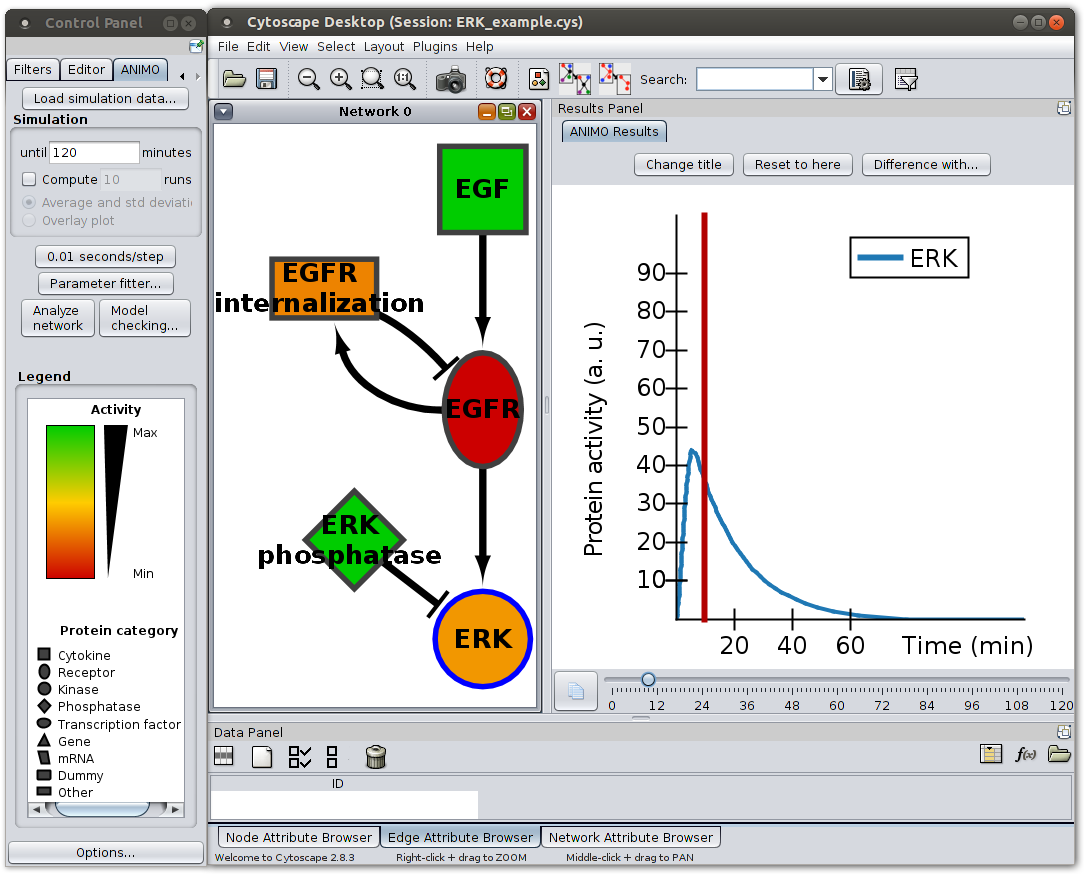
\includegraphics[width=.59\textwidth]{images/animo-ui}
  \caption{ANIMO user interface.\label{fig:animo-ui}}
\end{center}
\end{figure}

\begin{figure}[htbp]
\begin{center}
  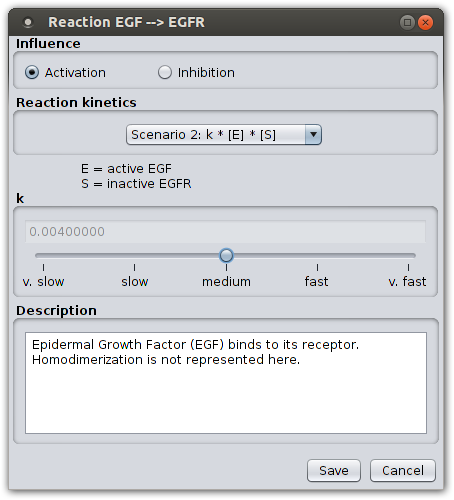
\includegraphics[width=.4\textwidth]{images/animo-edge-ui}
  \caption{Editing the parameters for an ANIMO interaction.\label{fig:animo-edge-ui}}
\end{center}
\end{figure}



Of the two main components of an ANIMO model, only the topology is immediately visible to the user in the
Network panel; the parameters are accessed by double clicking the arcs representing node-node interactions.
The dialog window that is shown for an interaction contains the details of the abstract reaction kinetic
describing the interaction, together with the current value of its parameter $k$ (see Fig.~\ref{fig:animo-edge-ui}).
The unique parameter associated to any interaction in ANIMO is used as a scale factor to make the modelled
reaction occur faster or slower. We also provide the user with pre-set values for
$k$, encouraging an initial qualitative assignment of reaction rates as ``slow'', ``fast'' and so forth.
This approach is based on the assumption that biological networks are inherently robust:
once an acceptable set of parameters is found, a more precise parameter search will generally have
little impact on the fitness of a model to a reference data set.
However, as can be seen in the small example in Figure~\ref{fig:small-example-feedback},
robustness does not imply that any parameter choice will do.
In that example, all parameters are initially set to \emph{medium}
(Fig.~\ref{fig:small-example-feedback}{\sf a}).
The peak in EGFR was obtained setting the value of $k$ for {\sf EGFR internalization}~$\dashv$~{\sf EGFR}
to \emph{fast} (Fig.~\ref{fig:small-example-feedback}{\sf b}). As this is not enough
to get a peak also for ERK, which remains constantly inactive, a lower value of $k$
for {\sf ERK phosphatase}~$\dashv$~{\sf ERK} can be tried. A first attempt with
\emph{slow} (Fig.~\ref{fig:small-example-feedback}{\sf c}) leads to a low peak,
which can be increased by further lowering that parameter to \emph{very slow}
(Fig.~\ref{fig:small-example-feedback}{\sf d}). Further adjustment of the parameters
and non-default scenario choices leads to the graph shown in Figure~\ref{fig:animo-ui}.
Network motifs such as the feedback loop shown in Figure~\ref{fig:small-example-feedback}
make models more dependent on parameter settings.
As biological networks tend to heavily rely on cross-talk, network topologies can rapidly become
complex. Some manual parameter fitting is currently necessary for the more complex ANIMO models.
This work is sometimes slow and error-prone, taking away some of the user-friendliness
for which ANIMO aims.
We will show how ANIMO has been improved to make parameter choice easier for the user.

\def\graphHeight{0.19\textheight}
\begin{figure}
%Show example on parameters of feedback inactivation loop (also the example ABCDE from ANIMO's manual would be ok)
%maybe changing the names to EGF, EGFR, EGFR intern, ERK, ERK phosph
\centering
%\begin{picture}(250,500)
%\put(0, 250){
\begin{tabular}{ccccccc}%
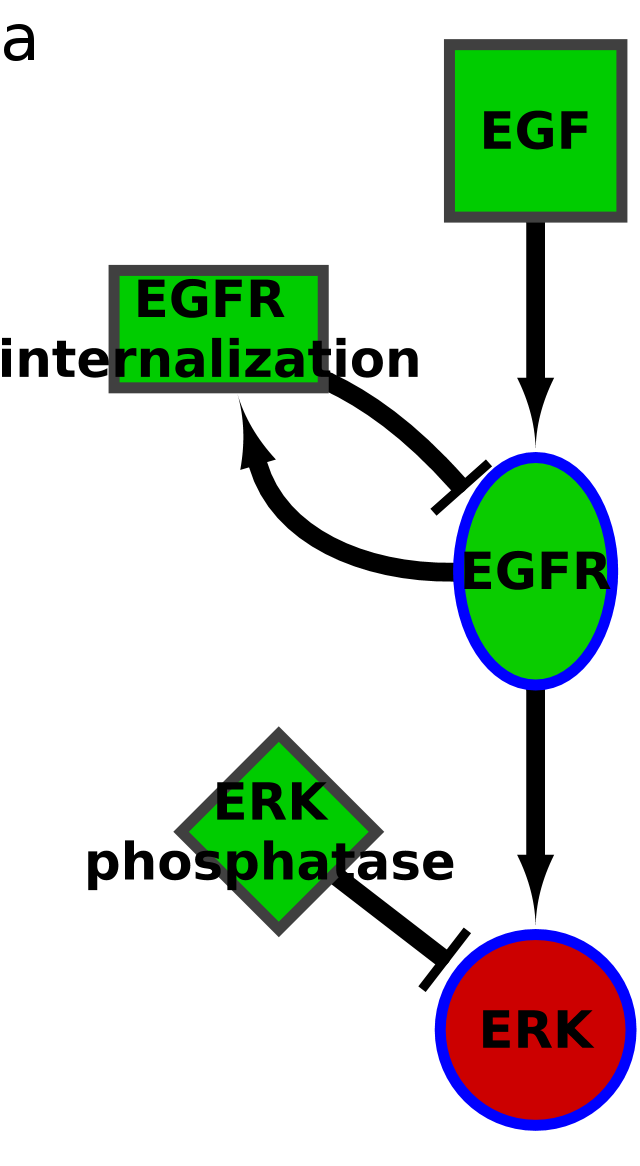
\includegraphics[height=\graphHeight]{images/feedback_params_netA} & \quad & 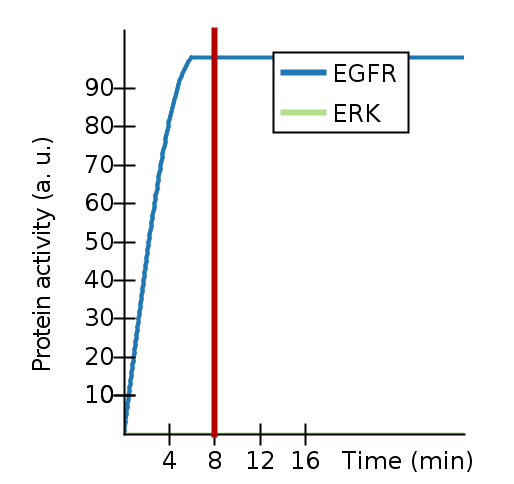
\includegraphics[height=\graphHeight]{images/feedback_params_graphA} &\quad&
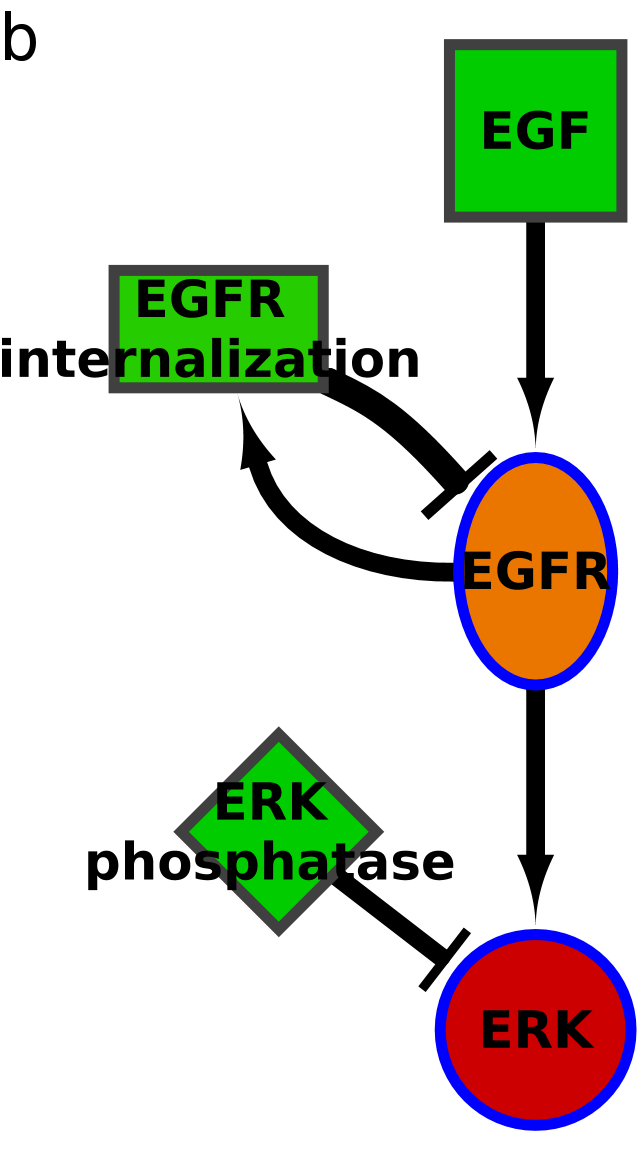
\includegraphics[height=\graphHeight]{images/feedback_params_netB} & \quad & 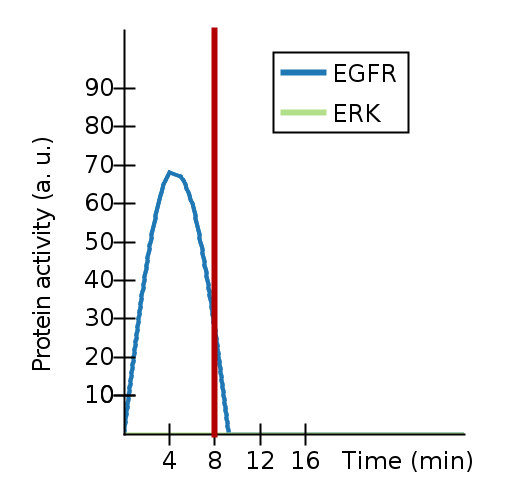
\includegraphics[height=\graphHeight]{images/feedback_params_graphB} \\
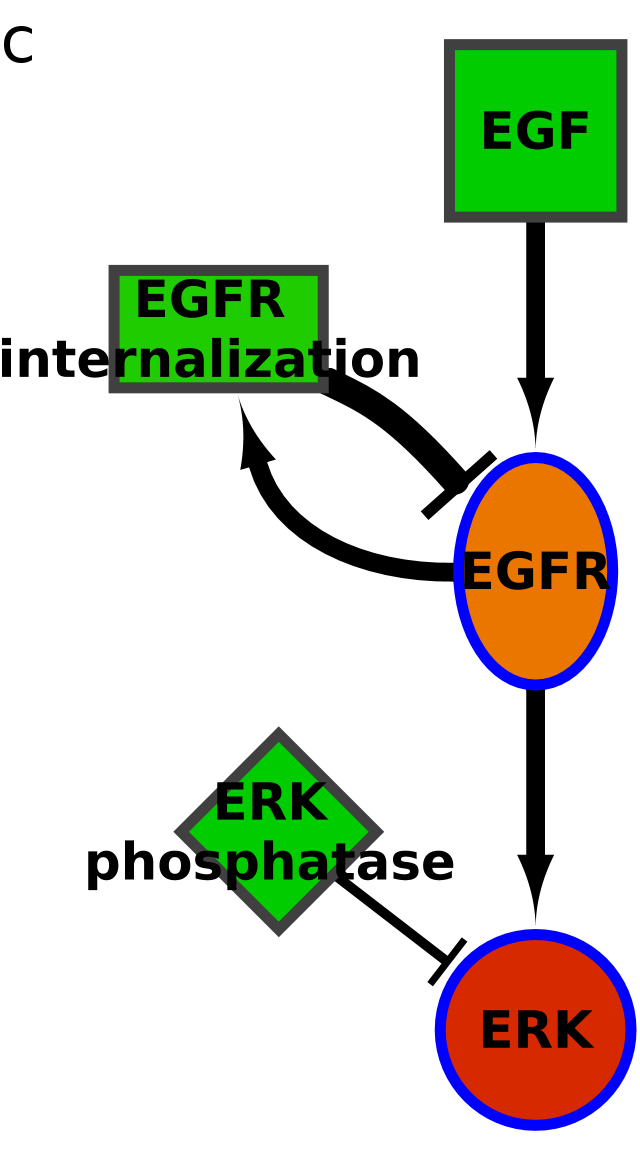
\includegraphics[height=\graphHeight]{images/feedback_params_netC} & \quad & 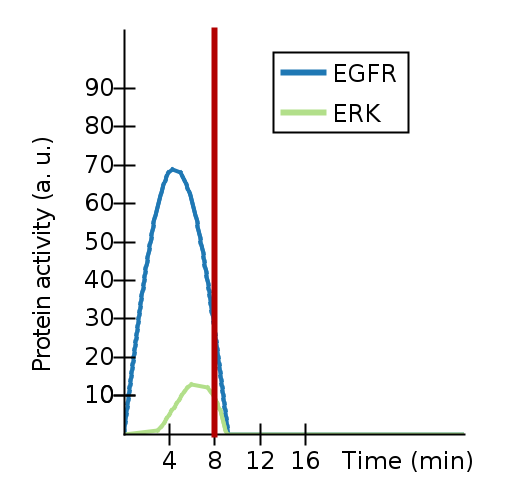
\includegraphics[height=\graphHeight]{images/feedback_params_graphC} &\quad&
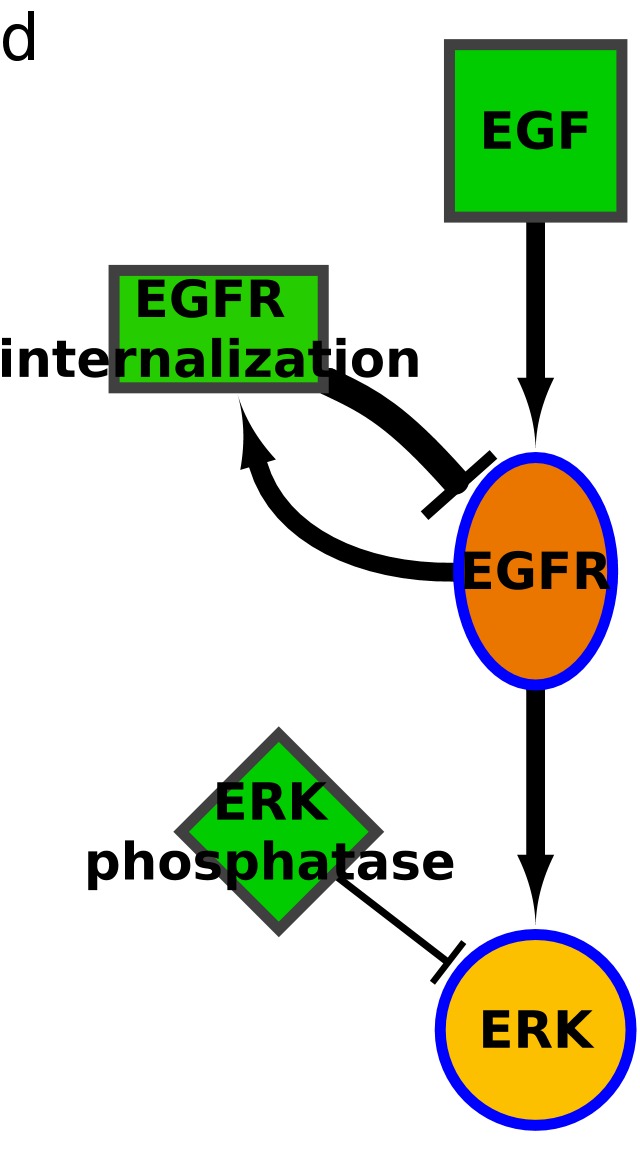
\includegraphics[height=\graphHeight]{images/feedback_params_netD} & \quad & 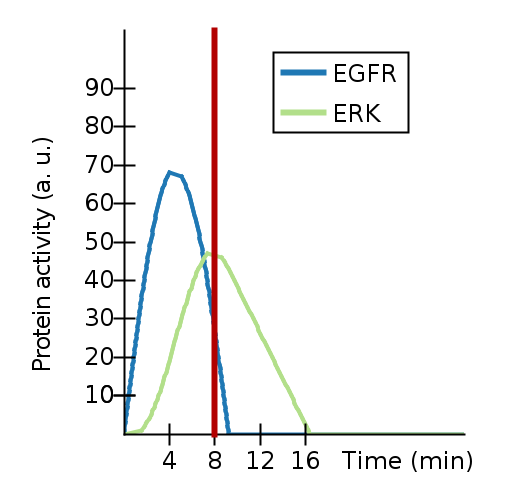
\includegraphics[height=\graphHeight]{images/feedback_params_graphD} \\
\end{tabular}\ \\
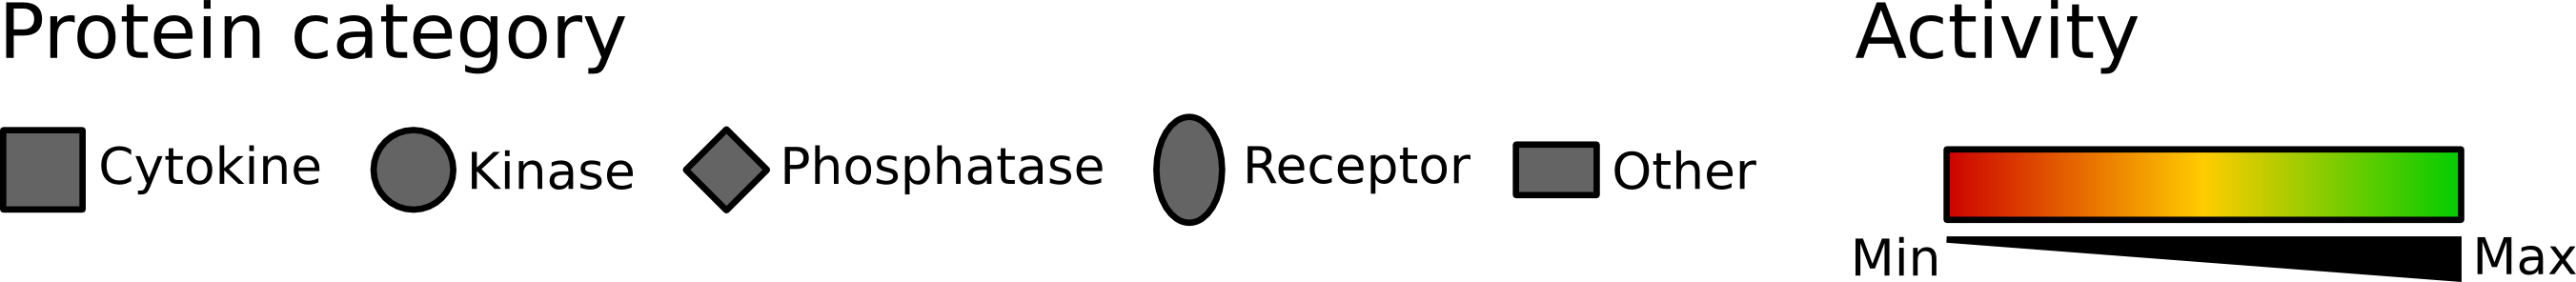
\includegraphics[width=0.8\textwidth]{images/legenda_forme_e_colori}%}
% \put(0, 220){
\includegraphics[width=0.5\textwidth]{images/dummy_sign}}
%\end{picture}
\caption{Example parameter settings on a simple feedback network.
Arc width on the left represents parameter values: thicker arcs correspond to higher values.
Colors on the left represent node activities at the points in time highlighted by the vertical
red lines in the corresponding graphs on the right.\label{fig:small-example-feedback}}
\end{figure}

% - slow/medium/fast..
% - parameter sweep
% - compare simulations
% Anche come sono fatti (esempio, parameter sweep: la formula dell'errore etc)
\section{Support for parameter synthesis in ANIMO}
When a model does not match experimental data, ANIMO offers three main tools to achieve a better fit:
manual parameter editing, comparisons between different model versions, and the newly introduced parameter sweep.

\subsection{Manual parameter editing}\label{sec:parameter-editing}
Double-clicking on an arrow in the Cytoscape representation of an interaction lets the user access
a dialog that allows to change the approximated scenario and parameters for the selected interaction.
The simplified scenarios were described in detail in~\cite{animo-ieee}, here a rough introduction is given.

In ANIMO, the \emph{activity level} of a reactant is a discrete value representing
the ``active'' fraction of a molecular species. For example,
a phosphorylated kinase is usually considered to be active, while its non-phosphorylated state
is considered inactive. The activity level is expressed in ANIMO with an integer value between
0 (completely inactive) and a maximum value that represents complete activity. The maximum value can
be chosen by the user on a range between 1 and 100, determining the granularity (or precision)
with which the activity of the reactant is represented in the model. For example, an ANIMO node
with 2 levels of granularity (thus with maximum activity set to 1) can be used to represent a gene, which is considered as either
completely active or completely inactive. A more precise representation of the activity level
is necessary when we want to represent more complex dynamics, where also intermediate values are considered
important. The activity level of a node can be changed in an ANIMO model by way of activations
and inhibitions, which make it respectively rise and decrease. Each occurrence of an abstract
interaction changes the activity level of the downstream node by 1 step. For example,
consider the interaction MEK $\rightarrow$ ERK, which represents the activation of ERK by (active) MEK.
Each time that interaction occurs, the activity level of ERK rises by 1: if ERK has 100 activity levels,
it will take 100 interactions to take it from full inactivity to full activity. The rate
at which such interactions will occur is determined by the scenario and parameter of the
interaction.

The scenarios are used to choose which are the nodes to be taken into account
when computing the speed at which an interaction occurs.
\begin{description}
  \item[Scenario 1] the simplest of the three, this scenario approximates an interaction
    without taking into account the abundance of substrate: the activation/inhibition rate
    depends only on the activity level of the upstream node. In the MEK $\rightarrow$ ERK
    example, the rate of the interaction would be linearly dependent on the current activity level of MEK.
  \item[Scenario 2] scenario 2 models the interaction rate
    to be directly dependent both on the activity
    level of the upstream node and on the availability of substrate. By substrate we
    mean the inactive downstream node in case of activation interaction, and active downstream node in case of inhibition.
    In the above example, the interaction rate is linearly dependent on
    both the activity level of MEK and the inactive fraction of ERK.
    The inactive level of a node is computed by subtracting the current activity level from the maximum activity.
  \item[Scenario 3] the nodes on which this scenario depends can be chosen directly by the user,
    and can be either the active or inactive fraction of any two nodes in the network.
    This scenario can be used to represent an AND-gate, where two nodes are required to
    be simultaneously active in order to influence their target.
\end{description}

The choice for the parameter $k$ can be made directly by inserting a numeric value, or 
indirectly by choosing a preset among the proposed qualitative values \emph{very slow, slow, medium, fast, very fast}.
% We advise our users to base their initial parameter choice on these qualitative presets.


\subsection{Comparing model versions}\label{sec:comparing-versions}
Particularly large networks make it more difficult for the user to understand the effects
of a change in network topology or interaction parameters. To overcome this difficulty, ANIMO
allows the user to visually compare two versions of a model in terms of their simulation results.
The Results panel in Figure~\ref{fig:animo-ui} shows the graph of selected node activities during
the course of an ANIMO simulation. The button labelled ``Difference with\dots'' allows to compare the current
simulation data with another based on a possibly different version of the model. When the two
simulations to be compared have been chosen, ANIMO produces a new graph plotting the difference
between the two original simulations. The slider under the new graph allows to visualize also
in the Network panel the changes in node activity in the whole network: Figure~\ref{fig:diff}
shows the difference between the first and last version of the model in Figure~\ref{fig:small-example-feedback}:
the difference was computed as {\sf d - a}. Nodes colored in green in the Network panel are
more active in version {\sf d}, while red nodes are more active in version {\sf a}.

\begin{figure}
\centering
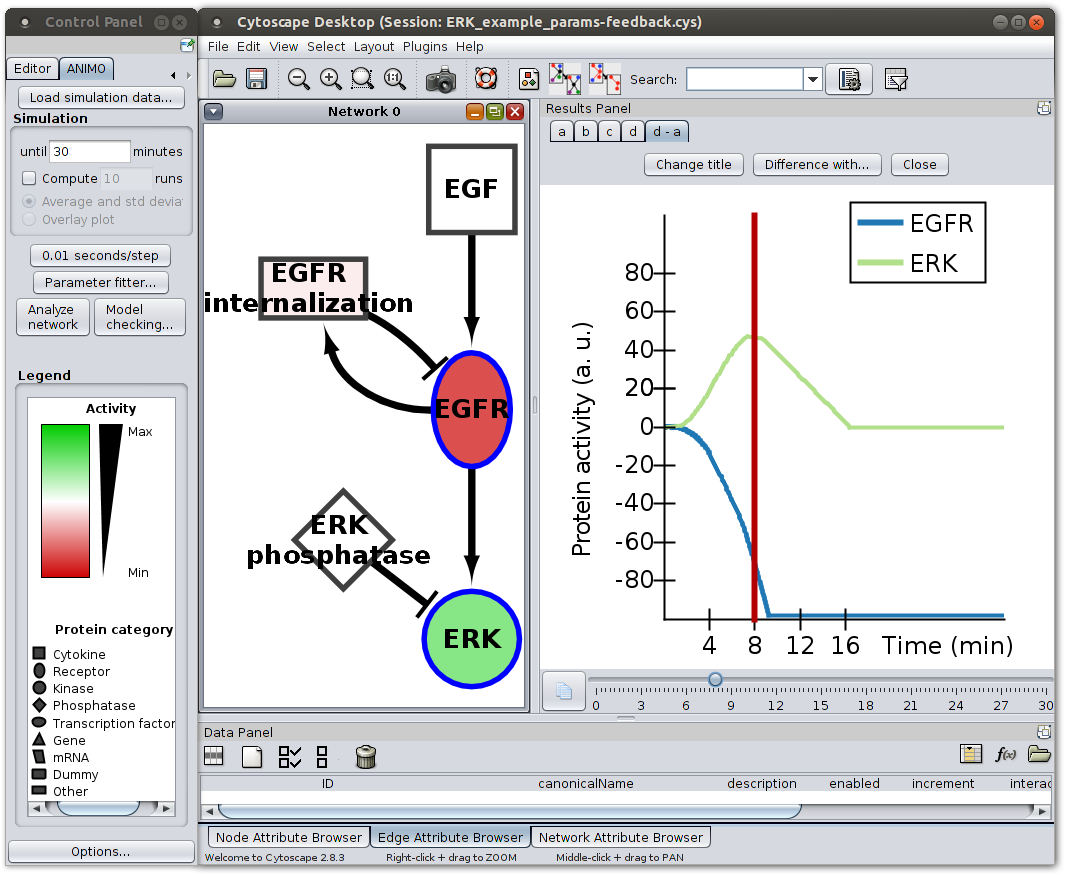
\includegraphics[width=.65\textwidth]{images/difference_network_d-a_larger}
\caption{Difference between the graphs in Figures~\ref{fig:small-example-feedback}{\sf a}
and~\ref{fig:small-example-feedback}{\sf d}. The Network panel shows the activity difference
in the network topology at the chosen simulation point represented by a vertical red line on the graph
in the Result panel.\label{fig:diff}}
\end{figure}


By changing the title of a simulation, a user can keep track of different versions of their model,
which can be also kept and saved with the model, to be used in future sessions or for sharing purposes.
Should a user want to backtrack to a particular version of the network, the ``Reset to this'' button
can be used. As an additional help to recall what a model version consisted of, the tooltip of
the ``Reset to this'' button shows an image of the network topology, taken in the moment when
the selected simulation was begun. A click on the ``Reset to this'' button will reset the
network topology and parameters at the ones used to generate the selected simulation.
As the adaptation of a model may proceed on different paths, the ``Difference with\dots'' and
``Reset to this'' buttons provide the user with some help with tracking the changes to the model
and selecting the most promising ones.

\subsection{Parameter sweep}\label{sec:parameter-sweep}
In order to avoid introducing too many changes to the topology of a network, ANIMO users
should be reasonably sure that a topology does not fit a given data set before
modifying the structure of the network. As this would entail an extensive parameter search which,
even with the tools
described in Sections~\ref{sec:parameter-editing} and~\ref{sec:comparing-versions}, would
require a considerable amount of time and effort, we have provided the latest version of ANIMO
with a support for parameter sweeps. The idea is to let ANIMO automatically explore a user-defined parameter
space by computing a series of simulations based on a constant network topology, where only the
parameters are being changed. Comparing the results with a given experimental data series
will allow for an automatic pre-screening, leaving the user with a choice among the best
fitting settings.
% Multicore!
Moreover, the task of parameter sweeping can be trivially parallelized, allowing us to
exploit the multi-core architectures available in most personal computers, and present the
users with the requested results in considerably less time.
In our case, the multi-core parameter sweep is implemented by using a thread pool pattern~\cite{thread-pool},
relying on the local scheduler to have the threads distributed on all CPU cores.

% log e linear scale
% error vs data --> narrower parameter choices
Another important option provided in ANIMO is the choice between linear and logarithmic scales
when defining the way a parameter space has to be explored: this gives the user more
control on the balance between precision and performances. When considering a big set of
interactions or of parameter settings, it is faster to proceed in logarithmic steps. After
a more precise interval of parameters has been identified for a subset of the interactions,
a linear search becomes more feasible. In this way, the computational resources can be used more efficiently
and results can be obtained faster.

The goodness of a model configuration is determined in ANIMO by comparing the activity graph
resulting from a simulation with the selected configuration
against a given experimental data set, applying the following formula for each of the selected data series $i$:
$$
\mbox{\it Error}_i = \max_{t = 0}^{\mbox{\it \scriptsize maxTime}} \frac{|\mbox{\it Data}_i(t) - \mbox{\it Model}_i(t)|}{\mbox{\it nLevels}_i}\\
$$
where $\mbox{\it Data}_i(t)$ is the experimental data point at time $t$ for the series $i$, 
$\mbox{\it Model}_i(t)$ is the corresponding value on the graph computed by ANIMO
with the current parameter configuration, and $\mbox{\it nLevels}_i$
is the granularity (number of levels) of the network node $i$.
The error of the given model configuration is then computed as the maximum error over
all selected data series:
$$
\mbox{\it Error} = \max_{i = 0}^{\mbox{\it \scriptsize nSeries}}(\mbox{\it Error}_i)
$$

% Si puo' anche valutare parameter sensitivity con questo metodo
Thanks to the support for parameter sweeps, ANIMO users can obtain better insight on the
parameter sensitivity of their models, identifying critical points in the networks.
% Such analyses could be performed in a Montecarlo-like fashion: first perform a sweep on
% (a large part of) the network using a logarithmic scale, then sweep separate subsets
% of interactions with more precise linear scale.
This can help identifying the most sensitive
areas of a network, and possibly suggest some intervention points for successive topology expansions,
if model robustness needs to be enforced. Note that the approach is only sketched here:
statistical considerations on confidence should also be taken into account.
% Infine, parameter sweep e' utile anche per simulare la variabilita' tra gli individui,
%  (e quindi accertarsi che il modello sia effettivamente robusto)

All the simulations computed in ANIMO when performing a parameter sweep are based on
a deterministic version of the model: a given parameter configuration gives always the same
simulation as result. This is why we use only one simulation per configuration
when comparing the results with experimental data. However, the user can add some
non-determinism to the model by defining uncertainty intervals around which interaction
times are distributed. For example, the default setting of 5\% uncertainty illustrated in~\cite{animo-ieee}
implies that an interaction can complete in a time $t$ sampled from an uniform distribution
in the continuous interval $[0.95 \times T, 1.05 \times T]$.
Here, $T$ is the exact time for one interaction step, and is computed by applying
the selected scenario to the current activity levels of the nodes involved in the interaction.
Adding uncertainty to a model can be used to test its robustness. The user can then
ask ANIMO to compute a number of simulations in \emph{overlay} mode,
which will allow the user to see all the simulations superposed in one graph,
and realize whether in some cases the model significantly deviates from its normal behavior.

% Concludi con esempio di sweep sull'esempio abcd (erk etc): son 3125 simulazioni se lo fai
%  andare solo sui parametri ``slow'', ``medium'', etc e con le 5 interazioni di abcde
We now present an example application of ANIMO's parameter sweep feature on the model shown in Figure~\ref{fig:animo-ui}.
Thanks to parameter sweep, we can make a more exhaustive search than the one presented in Figure~\ref{fig:small-example-feedback},
using an automatic approach instead of a manual trial-and-error process.
A logarithmic parameter sweep was performed, letting the parameter values
vary over the 5 pre-sets ``very slow'' ($k = 0.001$), ``slow'' ($k = 0.002$), ``medium'' ($k = 0.004$), ``fast'' ($k = 0.008$), ``very fast'' ($k = 0.016$)
for all 5 interactions in the network. This resulted in $\mbox{\it parameter choices}^{\mbox{\it\scriptsize interactions}} = 5 ^ 5 = 3\,125$ simulations, that were computed
in 43 seconds %43 s with 16 threads. It is 57 with 8 threads (cpu is exploited less than 100%)
on an eight-core Intel\circledR\ Core$^{\mbox{\scriptsize\texttrademark}}$ i7 CPU at 2.80GHz equipped with 4 Gb RAM
and running Ubuntu GNU/Linux 13.10 64bit. The model we consider here is small enough for one simulation to take
less than a second, but the exponential growth of the number of simulations required for a parameter sweep
can make the sheer number of tasks challenging for any processing unit.
% Indeed, a more thorough
% parameter sweep that considers 10 different setting for each of the 5 interactions of the considered
% model would require the computation of $10^5 = 100\,000$ simulations.
For example, a more complex model involving 10 interactions instead of 5 would require $5^{10} = 9\,765\,625$ simulations,
which could be computed in approximately a day and a half on an eight-core machine.
Still, the possibility to compute simulations in parallel provides a significant help in reducing
the impact of an exponential growth of the space to be explored.
% Yet, such an
% estimation would still be better than the twelve days it would take if the simulations were to be computed in sequence.
% the same experiment
% was run executing only one simulation at a time, and it took about 7 minutes and 34 seconds, %453837 ms
% which is in line with the fact that this type of analysis is trivially parallelizable.

The result window shown by ANIMO at the end of the computation of the $3\,125$ simulations can
be seen in Figure~\ref{fig:parameter-sweep-result}, where the best 6 results are listed in form of graphs.
By interacting with the interface, the user can choose to see more of the top-scoring results: this will allow to check
the width of the parameter settings for which the wanted behavior can still be considered ``close enough'' to
the experimental data. Pressing one of the buttons labelled ``I want this'' under one of the graphs
allows the user to copy the parameters used in the selected simulation to the network model.

% We note that all scenarios for the 5 interactions were set to the basic scenario 1 for this parameter
% sweep. The graph can be made fit the actual data more precisely by selecting scenario 2 settings for some
% of the interactions. The choice of a scenario has little to no impact on the complexity of the model:
% after choosing scenario 2 for all of the interactions, the whole parameter sweep takes the same time to complete.

\begin{figure}
\centering
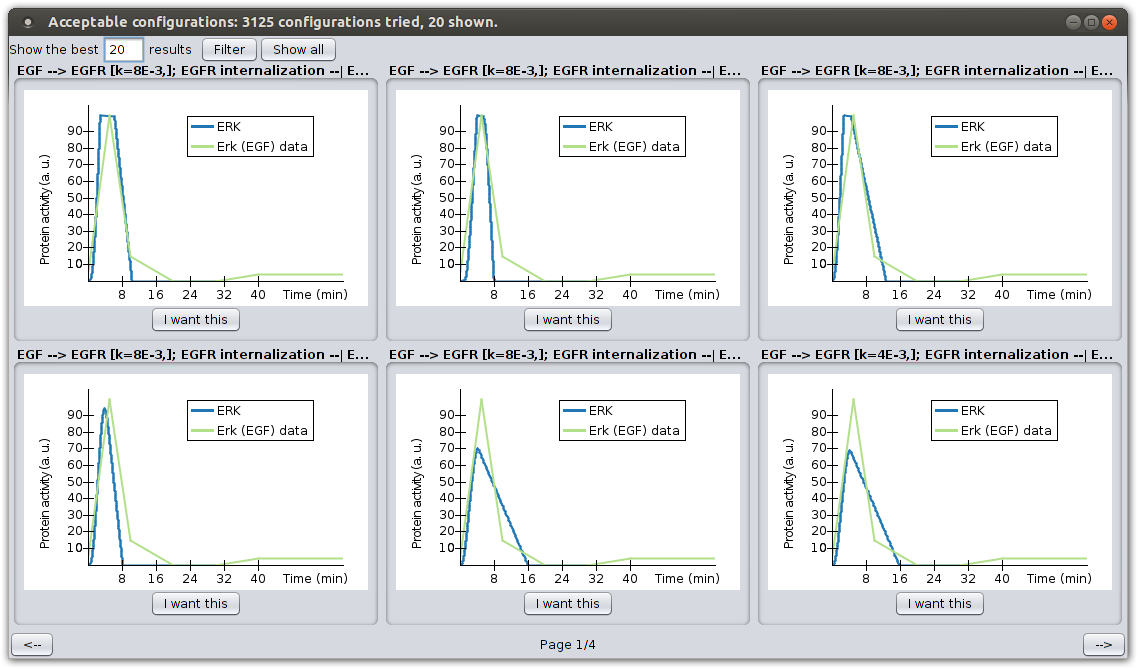
\includegraphics[width=0.92\textwidth]{images/parameter_sweep_results}
%\begin{picture}(350,260)
%\put(0, 0){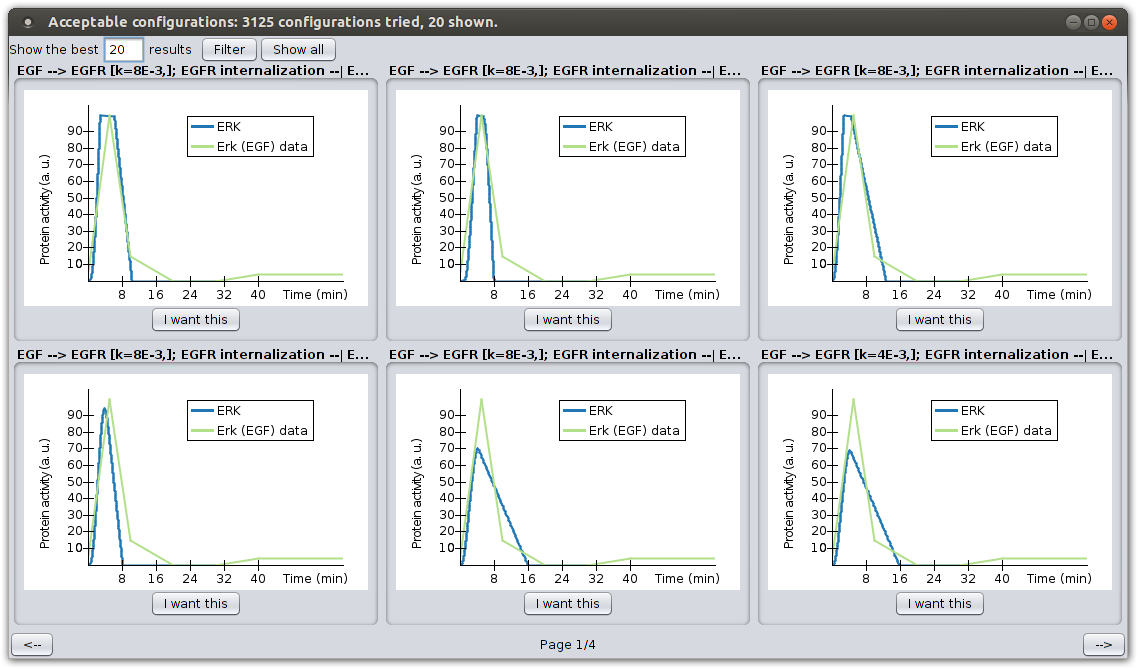
\includegraphics[width=0.8\textwidth]{images/parameter_sweep_results}}
%\put(150,50){\hbox{Over here}}
%\put(70, 70){
\includegraphics[width=0.5\textwidth]{images/dummy_sign}}
%\end{picture}
\caption{Result window of a logarithmic parameter sweep in the ANIMO model of Figure~\ref{fig:animo-ui}.\label{fig:parameter-sweep-result}}
\end{figure}


% dopo aver presentato gli strumenti che forniamo, definiamo una procedura consigliata per usare ANIMO nel modo pi� efficace.
% Ovviamente, oltre alle best practices serve anche l'esperienza, sia intesa come conoscenza di biologia che come esperienza
% nel campo della modellazione. Nota che non serve comunque conoscenza di T.A., visto che rimangono sempre nascosti dietro la GUI
% Esempio/case study!
\section{Suggested ANIMO workflow}
In order to better profit from what ANIMO offers to the biologist, we suggest a step-by-step modeling workflow:
\begin{enumerate}
  \item\label{step:def-topology} Define a starting topology, based on literature data and current knowledge on the network.
  \item\label{step:set-rates} Choose the interaction parameters from the pre-set qualitative values,
    based on experience (e.g., protein expression is much slower than phosphorylation).
    The choice on the approximated kinetics can be for the most part based on scenario 1, referring to Section~\ref{sec:parameter-editing}.
  \item\label{step:check-behavior} Check that the network behaves as expected (e.g. addition of EGF makes ERK activity rapidly increase and successively decrease).
  \item Possibly iterate the steps~\ref{step:def-topology} to~\ref{step:check-behavior} until the network behaves as expected.
  \item Compare the model with experimental data.
  \item\label{step:precise-fit} If the model does not fit the data, change the parameters using more precise numerical values and/or scenario settings.
  \item\label{step:param-sweep} If the data fitting is still not satisfactory, apply parameter sweep to (subsets of) the model as described in Section~\ref{sec:parameter-sweep}.
  \item When a good fit is found, add non-determinism to the model and ensure that the
     behavior does not change significantly under reasonably high uncertainty settings.
  \item If the model can fit the data only with very precise parameter settings, or a
    parameter configuration that fits the data cannot be found after a reasonably extensive search
    on the parameter space, change the network topology possibly adding more nodes from literature.
    If no candidates can be found in literature, speculative candidates can be found by ``playing'' with the current
    configuration in ANIMO's user interface.
    We advise to let expert biologists perform this step on their own, or to perform it under their supervision,
    in order to keep the network both simple and realistic. For the same reason, we also advise not to introduce more than a couple of nodes at a time.
  \item Parameters for newly introduced interactions can be chosen as in step~\ref{step:set-rates}, possibly iterating
    steps~\ref{step:def-topology} to~\ref{step:param-sweep} to refine the parameters.
  \item To check how changes in the network are reflected in the behavior of the model, we advise to use the comparison tools
    described in Section~\ref{sec:comparing-versions}.
  \item When a model is obtained that behaves more closely to the experimental data,
  its fitness can be improved going back to step~\ref{step:precise-fit}.
\end{enumerate}
If the model fits the data reasonably well only after modifications to the initial topology, it may contain some hypothetical or unexpected nodes.
In that case, future experiments can be derived directly from the hypotheses introduced in the model and
help the biologists decide which are the most precise explanations for the experimental observations.

In general, the process described above allows the biologists to formalize their knowledge,
and makes it easier to have group discussions when trying to combine multiple subnetworks in a more comprehensive model.
It is worth noting that experience in both the specific biological setting and generic modeling of biological
events represents an important asset for a faster and more realistic modeling process with ANIMO. However, as
we claimed with all previous versions of the tool, it is still the case that no experience in formal methods
is needed in order to use ANIMO. In particular, an ideal ANIMO user could have no experience on the \tas\ foundations
of the tool and yet fully profit from its features.

% anche Related work: es. Copasi
% Altro su parameter sweep/sensitivity analysis? Noi usiamo un approccio un po' naif, senza tante pretese, senza tanti numeri.
% Possibile future work: vedere meglio altri modi di applicare parameter setting nel contesto dei t.a., usare
% calcolo distribuito per accelerare la ricerca dei parametri
\section{Conclusions}
ANIMO has been extended with a proper support for parameter synthesis. Now the tool can be used more efficiently
to model biological networks, without concentrating exclusively on their topology.
In particular, the addition of an automatic parameter sweep feature allows the user
to save considerable amounts of time, keeping closer to experimental data without the disadvantages
coming from a hand-made parameter search.

% \section{Bibliography}
% 
% We request that you use
% \href{http://www.cse.unsw.edu.au/~rvg/EPTCS/eptcs.bst}
% {\tt $\backslash$bibliographystyle$\{$eptcs$\}$}
% \cite{bibliographystylewebpage}. Compared to the original {\LaTeX}
% {\tt $\backslash$biblio\-graphystyle$\{$plain$\}$},
% it ignores the field {\tt month}, and uses the extra
% bibtex fields {\tt eid}, {\tt doi}, {\tt ee} and {\tt url}.
% The first is for electronic identifiers (typically the number $n$
% indicating the $n^{\rm th}$ paper in an issue) of papers in electronic
% journals that do not use page numbers. The other three are to refer,
% with life links, to electronic incarnations of the paper.
% 
% Almost all publishers use digital object identifiers (DOIs) as a
% persistent way to locate electronic publications. Prefixing the DOI of
% any paper with {\tt http://dx.doi.org/} yields a URI that resolves to the
% current location (URL) of the response page\footnote{Nowadays, papers
%   that are published electronically tend
%   to have a \emph{response page} that lists the title, authors and
%   abstract of the paper, and links to the actual manifestations of
%   the paper (e.g.\ as {\tt dvi}- or {\tt pdf}-file). Sometimes
%   publishers charge money to access the paper itself, but the response
%   page is always freely available.}
% of that paper. When the location of the response page changes (for
% instance through a merge of publishers), the DOI of the paper remains
% the same and (through an update by the publisher) the corresponding
% URI will then resolve to the new location. For that reason a reference
% ought to contain the DOI of a paper, with a life link to corresponding
% URI, rather than a direct reference or link to the current URL of
% publisher's response page. This is the r\^ole of the bibtex field {\tt doi}.
% DOIs of papers can often be found through
% \url{http://www.crossref.org/guestquery};\footnote{For papers that will appear
%   in EPTCS and use \href{http://www.cse.unsw.edu.au/~rvg/EPTCS/eptcs.bst}
%   {\tt $\backslash$bibliographystyle$\{$eptcs$\}$} there is no need to
%   find DOIs on this website, as EPTCS will look them up for you
%   automatically upon submission of a first version of your paper;
%   these DOIs can then be incorporated in the final version, together
%   with the remaining DOIs that need to found at DBLP or publisher's webpages.}
% the second method {\it Search on article title}, only using the {\bf
% surname} of the first-listed author, works best.  
% Other places to find DOIs are DBLP and the response pages for cited
% papers (maintained by their publishers).
% {\bf EPTCS requires the inclusion of a DOI in each cited paper, when available.}
% 
% Often an official publication is only available against payment, but
% as a courtesy to readers that do not wish to pay, the authors also
% make the paper available free of charge at a repository such as
% \url{arXiv.org}. In such a case it is recommended to also refer and
% link to the URL of the response page of the paper in such a
% repository.  This can be done using the bibtex fields {\tt ee} or {\tt
% url}, which are treated as synonyms.  These fields should not be used
% to duplicate information that is already provided through the DOI of
% the paper.
% You can find archival-quality URL's for most recently published papers
% in DBLP---they are in the bibtex-field {\tt ee}. In fact, it is often
% useful to check your references against DBLP records anyway, or just find
% them there in the first place.
% 
% When using {\LaTeX} rather than {\tt pdflatex} to typeset your paper, by
% default no linebreaking within long URLs is allowed. This leads often
% to very ugly output, that moreover is different from the output
% generated when using {\tt pdflatex}. This problem is repaired when
% invoking \href{http://www.cse.unsw.edu.au/~rvg/EPTCS/breakurl.sty}
% {\tt $\backslash$usepackage$\{$breakurl$\}$}: it allows linebreaking
% within links and yield the same output as obtained by default with
% {\tt pdflatex}. 
% When invoking {\tt pdflatex}, the package {\tt breakurl} is ignored.

%\nocite{*}
\bibliographystyle{eptcs}
\bibliography{Paper}
\end{document}
